\chapter{Literature review}
\section{The Enigma Machine}
\begin{figure}[hbt!]
    \centering
    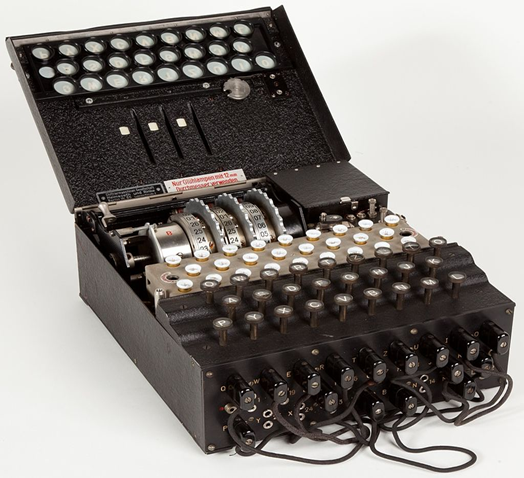
\includegraphics[width=0.6\linewidth]{myReport//figures/Enigma_icon.png}
    \caption{An “Enigma I” cipher machine with a clear showcase of rotors, plugboard, keyboard, and light bulb for display (Source: wikipedia)}
    \label{fig:enter-label}
\end{figure}

Enigma is one of the most important cipher machines used before and during WWII. It was released for commercial use at the beginning and became the cipher used by the military with significant improvement. Enigma performs a form of polyalphabetic substitution cipher \cite{greydanus2017learning}. Although substitution ciphers cannot satisfy the modern standard of encryption, cryptanalysis on classical ciphers like Enigma is still a direction of modern cryptanalysis research. 

\begin{figure}[hbt!]
    \centering
    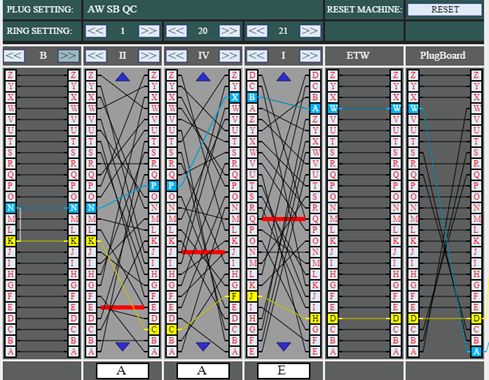
\includegraphics[width=0.6\linewidth]{figures/Enigma_emulator.png}
    \caption{Interface of an Enigma emulator, showing the substitution of each part of the Enigma}
    \label{fig:graph}
\end{figure}

The main structure of an Enigma machine that is related to encryption and decryption includes a set of rotors, a reflector, and a plugboard. The encryption and decryption operations of Enigma require the settings of each machine (sender and receiver) to be the same. Each time when a key is pressed down, the states of rotors would step by one. The electric signal would get through the plugboard, a set of rotors and a reflector. Each part of it would change the position of the electric signal.  The signal would pass through the plugboard and a set of rotors and reach the reflector, then the signal would be reflected and get through the Rotors and plugboard reversely. The final position of the signal would be displayed on the lamb board. This is the process of encrypting a single input character. The rotors “step” in a manner similar to an automobile's miles-meter. The rightest rotor steps 26 time between single steps of the next rotor, which is turn steps 26 times for each step of its neighbour on the left. The state of rotors would change and encrypt the next character in different substitution.


\begin{figure}[hbt!]
    \centering
    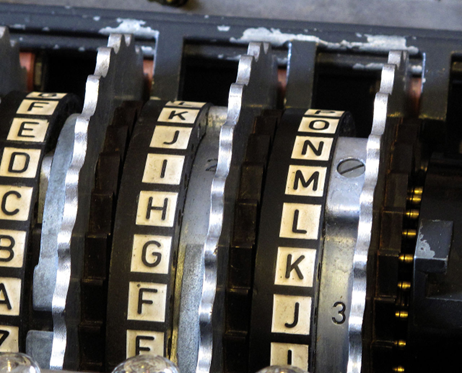
\includegraphics[width=0.5\linewidth]{figures/rotors.png}
    \caption{A closer view to Enigma's rotors}
    \label{fig:graph}
\end{figure}


Rotors are the core mechanism of encryption in the Enigma mechanism. During encryption, 3 to 4 rotors would be used and each rotor performs a layer of substitution on encryption depending on its types, rotor position and ring setting. The military model has 5 different types of replaceable rotors(marked as I, II, III, IV, and V). Each rotor has a different connection and turnover position. Each of them have a ring setting that change the connections by shifting. The position of the rotors are changed by stepping and turnover. Stepping is when a letter is pressed, one or more rotors would rotate to change the substitution of rotors. Each rotor has at least one turnover position, it shifted the position of next rotor for one. With every setting except the position of rotors fixed, a three rotors Enigma could provide 17576 (\(26^3\)) different combinations of substitution.

% \begin{figure}[ht]
% 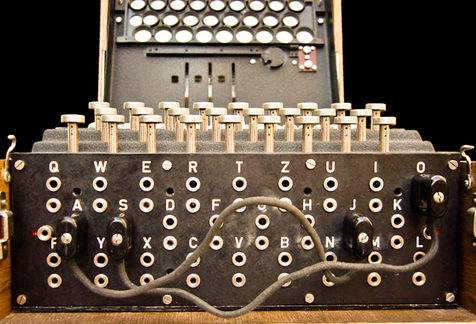
\includegraphics[width=15cm]{figures/plugboard.png}
% \caption{Enigma's plugboard connecting alphabet to others}
% \label{fig:graph}
% \end{figure}

The Plugboard is the major improvement from commercial Enigma to Military used Enigma. It was introduced to improve the strength of cryptographics since the Rotor only Enigma has been proved to be susceptible to manual analysis. The plugboard has the same amount of port as the alphabets. By connecting two alphabets, the inputs and the outputs of these two characters would be swapped. A plugboard provided a limited substitution layers. A certain numbers of character can be swapped. The remain characters are remain unchanged. 

The Reflector comes after the last rotor of the Enigma machine. It was introduced to make the Enigma reciprocal, which means it can encrypt and decrypt cipher in the same setting without swapping the mode. The reflector is usually fixed during the encryption, but in some of the models, the position of the reflector could be changed. 


\section{Cryptanalysis}

Cryptanalysis is to obtain information that could compromise the operation of a crypto system. This could include recovery of a secret key (or other secret interned approaches) or compromise of encrypted data recovery of plaintexts. This is also a form of attack to breach the system and the cryptographic systems and access to the encrypted messages without knowing part of the encryption requirements.  

\noindent\textbf{Classical cipher} \qquad		Classical ciphers cover the early history of the cryptographic and the majority of classical ciphers are often based on the substitution cipher. Some of the most representative ciphers are Caesar cipher, Vigenère cipher, and Enigma. The Caesar cipher is a monoalphabetic substitution cipher that applies a shift on the plaintext. For example, a Caeser cipher that shift the character for 3 step will encrypt the character “D” to “A” and “A” to “X”. The Vigenère cipher, which is a polyalphabetic substitution cipher, applies multiple substitutions on a single alphabet depending on the key's string. The Enigma machine is a mechanical cipher with more complexity than the previous two methods, but fundamentally it is still a polyalphabetic substitution cipher.

\noindent\textbf{Breaking classical ciphers	} \qquad	The works on breaking classical ciphers have a longer history as well. At the early stage of cryptanalysis, frequency analysis is a commonly used technique. Frequency analysis follows the assumption that in a natural language text, some of the word or character would have higher frequency. For example, the character “T” and word “THE” in English, the word “EIN” in German. If these patterns and characters were observed in decrypted text, then this is likely a successful decryption. The first known record of frequency analysis was presented by a 9th century polymath, AI-Kindi. His work was inspired by the Book of cryptographic messages. Frequency analysis method has a strong impact on the breaking of monoalphabetic ciphers and part of the polyalphabetic ciphers.
The classic cryptography had reached its peak at the Lorenz cipher and Enigma machines. During WWII, they took a huge amount of effort from codebreakers and mathematicians to break the cipher. The breaking of the Enigma and Lorenz cipher involves all known techniques of cryptanalysis. For example, codebreakers performed frequency analysis by observing some of the most frequent patterns in German, include the word ‘EIN’ (means ‘one’, ‘a’ in English) that mentioned before. Some of the weaknesses of Enigma were also exploited. Even so, there was a lot of effort spent outside of codebreaking. Knowledge of Enigma was also gained from operator mistakes, captured hardware and codebooks, and knowledge of commercial Enigma, etc. Without the knowledge from outside, understanding the functionality of Enigma would be an extremely challenging mission.

\section{Machine learning in cryptanalysis}

\begin{figure}[hbt!]
    \centering
    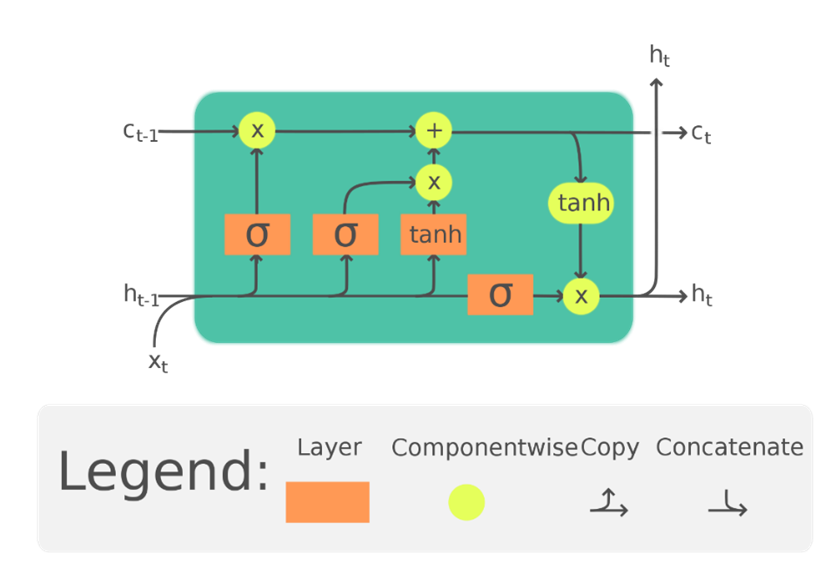
\includegraphics[width=0.8\linewidth]{figures/LSTM.png}
    \caption{A Long Short-Tern Memory Unit}
    \label{fig:graph}
\end{figure}

Substitution ciphers cannot satisfy the modern standards of cryptography because with more computation resources available, brute forcing is becoming easier than before. At the same time, machine learning also benefits from the computation resources. The machine learning field made a breakthrough in 2012 because of the strong performance and impressive production of deep convolutional neural networks. After that, deep learning becomes a well-researched field. It has been applied to fields like computer vision, natural language processing, data science, statistics, computational neuroscience, and cryptanalysis, which is what we are going to research in this project.



\noindent\textbf{Recurrent neural network (RNN)} \qquad		Recurrent neural networks are an important architecture in deep learning, mostly used for modelling the sequential data. This include speech, text, or even video. In the RNN, the neural network takes each token of sequences as inputs, and each token after first tokens would also take the previous output as input. This allows the information from previous tokens to make an influence on the next tokens. 
The main issue of the originally presented RNN is the gradient vanish problem. When the input sequence is long, the gradient might decrease to 0 after passing through long sequences. Two different forms of improvement have been made to address this problem. Long Short-Term memory was proposed in 1997 by Hochreiter et al \cite{hochreiter1997long}. LSTM introduced RNN with an input gate, output gate, and a cell of context. The network would learn how much information to transfer to the next token and how much information needs to be forgotten. This architecture has been proved to be successful in tasks like machine translation and speech recognition. In 2014, another network based on recurrent neural network, the Gated Recurrent Union was presented \cite{chung2014empirical}. This architecture uses a smaller number of gates based on the sigmoid function to control the flow of information. It contains fewer parameters than the LSTM model and can maintain similar performance. 

\begin{figure}[hbt!]
    \centering
    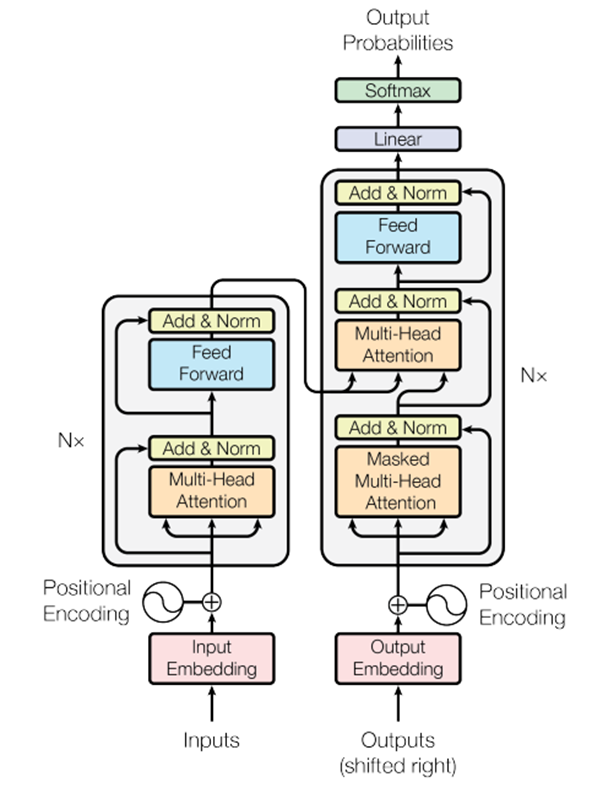
\includegraphics[width=0.5\linewidth]{myReport/figures/transformer.png}
    \caption{The transformer architecture. Presented by Vaswani et al\cite{vaswani2017attention}}
    \label{fig:graph}
\end{figure}

\noindent\textbf{Transformer} \qquad		The Transformer is a milestone of machine learning model. It was presented in 2017 by Vaswani et al \cite{vaswani2017attention} from Google Research. The Transformer was proposed for the machine translation task, then upcoming research extended its functionality to multiple different tasks in natural language processing, even computer vision and multimodality. Today, the transformer's decoder or encoder is the core part of machine translation and natural language generation AI. The most famous product by far is the GPT series model from OpenAI \cite{ouyang2022training}. The architecture of the Transformer is based on the self-attention mechanism and fully connected neural network. When compared with RNN families like LSTM, Transformer has the advantage of time complexity and scalability. It processes the entire sequence inputs at the same time by a single matrix multiply action. This allows Transformer to process the entire sequence in a single time of computation. The use of residual connection \cite{he2016deep} also helps the Transformer to have more layers and parameters. Positional encoding is introduced to inject the sequence information into Transformer because the transformer itself didn’t model the order of sequence. 


\noindent\textbf{Reinforcement learning} \qquad		Reinforcement learning is an area of machine learning that is different with majorities. It usually involves an Agent and an environment. And the reward and the state of the activities of the Agent would feedback to the agent for the Agent to optimise.

In cryptanalysis, brute forcing requires good thought of each different combination, and choosing the largest expected return. The issue is the number of combinations could be very large or even infinity and the computational complexity would also increase. Fitness function(value function estimation) helps the reinforcement learning to understand how much the behaviour of the agent has met the requirements and the direct policy search allows some of the generated behaviour to have influence on others. A reasonable choice of fitness function and direct policy search is more efficient than searching each possible combination or search completely randomly.

\section{Previous research}
\noindent\textbf{Genetic algorithms attack on Plugboard} \qquad		Sommervoll et al \cite{sommervoll2021genetic} illustrated the relation between Enigma and machine learning and the method of Genetic algorithms’ usage on attacking the plugboard of Enigma. The main contribution of this paper is the fitness function based on the similarity with natural language patterns. The paper’s assumption is based on the concept of IC(index coincidence). In the natural language, some of the alphabet has more frequency than others and in the randomly generated text, each alphabet has a similar appearance. By observation, the researcher found that the plaintext has an IC similar to natural language, and the encrypted ciphertext has an IC similar to the random generated plaintext. By this step, the paper presented a score function based on how similar the decrypted pattern was with a natural language pattern. For the genetic algorithms, the paper also illustrated the details of genes, and how the mutation and crossover of this attack is performed.

\noindent\textbf{Learn and attack the Enigma by RNN} \qquad		Greydanus et al’s \cite{greydanus2017learning} experiment mentioned their attempt on using Recurrent neural networks to learn and attack presentive classical ciphers. The paper trains RNN to learn three different ciphers (Autokey, Vigenère, Enigma) successfully. The paper also made attempts to train the RNN to recover key bits for all tested ciphers. The results show that RNN could learn the function of ciphers. However, for the cipher with higher complexity, like Enigma, the RNN used in the paper has 18,012,000 of parameters. This is too large for a model to learn substitution cipher. And it took more than a million pairs of plaintext and ciphertext to train. The result of attacking the key bits is also limited. The paper only showed some of the results on attacking the Vigenère and Autokey ciphers. The results for the Enigma cipher are absent.



\noindent\textbf{Machine learning on time series analysis/forecasting} \qquad		The Transformer has dominated and achieved great success in lots of natural language processing. However, it still has its weakness in temporal data, especially data that is influenced by time series \cite{lim2021time}. 
According to the definition, time series is a series of data listed in the time order. In machine learning competitions like Kaggle, the LSTM is still widely used in time series forecasting. Google also presented their LSTM and Transformer hybrid model Block Recurrent Transformer \cite{hutchins2022block} for tasks particularly related to time forecasting, designed to combine the advantages of two different architectures.
Enigma has its states stepped after each encryption of the alphabet. The substitution process in encryption would develop and change over the time. Attack and recovery of the states of Enigma could be viewed as a time series analysis task. In this case, according to the case we listed above, the Transformer might not be the best model in modelling time series model. Our experiment should cover different architectures to compare their performance.


\section{Summary}
Greydanus \cite{greydanus2017learning} et al's work was published in 2017, it didn’t apply the state-of-the-art architecture on learning and key recovery tasks. The model is also not scaled up in an efficient way (using bidirectional RNN, adding more layers). These led to in-efficient design in model architecture and training pipelines. By reading through the works on paper, we also noticed that there are some improvements we could make or try. These include the choice of loss function and the method to pre-process the inputs.
Issues mentioned above might be caused by the limitation of literatures and deep learning toolkits back then. Following the direction of the paper, with newly proposed machine learning techniques and deep learning toolkits. We could step further from the direction of the paper to explore if there are efficient methods for learning the cipher and attack the initial rotor position of the Enigma machine. In this project, we could make attempts to find methods to learn the cipher efficiently. And more importantly, we could find out methods to attack the key bits of the Enigma machine.

